\chapter{分析与改进}

\section{过采样vs欠采样}

之前我们使用的是直接拷贝原图片的过采样,这样一共生成了100w万张以上的单词图片,但其中大部分公式图片都是重复的,而且重复度非常高,这样不仅数据多样性低,而且十分容易过拟合,使得在测试集上效果变差。虽然论文图片中大部分都是单词,但单词之间差异远小于公式之间的差异,故我们可以采用欠采样,即在单词图片中随机抽取与公式图片等量的图片。欠采样大大减少了相同程度训练下的数据量,在同等数据量下则大大提高了数据的多样性。虽然导致单词的多样性降低了,但单词的特征本身就比公式特征要简单,故采用欠采样将极大地提高数据的合理性。我们使用欠采样生成了50万左右的单词图片,而使用的原始论文图片则远多于过采样所使用的数量。

\section{网络改进}
\noindent

在参考了AlexNet和VGGNet网络模型之后,结合自己的实际情况,测试时间有限,也没有服务器支持,故自行设计了一个相对简单的网络。网络一共10层,四层卷积层,两层池化层,两层全连接层和一层输出层,此外在最后一个卷积层和第一个全连接层之间加入了一层Spp,前面Spp-Net中也提到了spp层,网络结构如图3.1\footnote{\hbox{This figure is generated by adapting the code from https://github.com/gwding/draw\_convnet}}。
\begin{figure}[ht]
    \centering
    \hbox{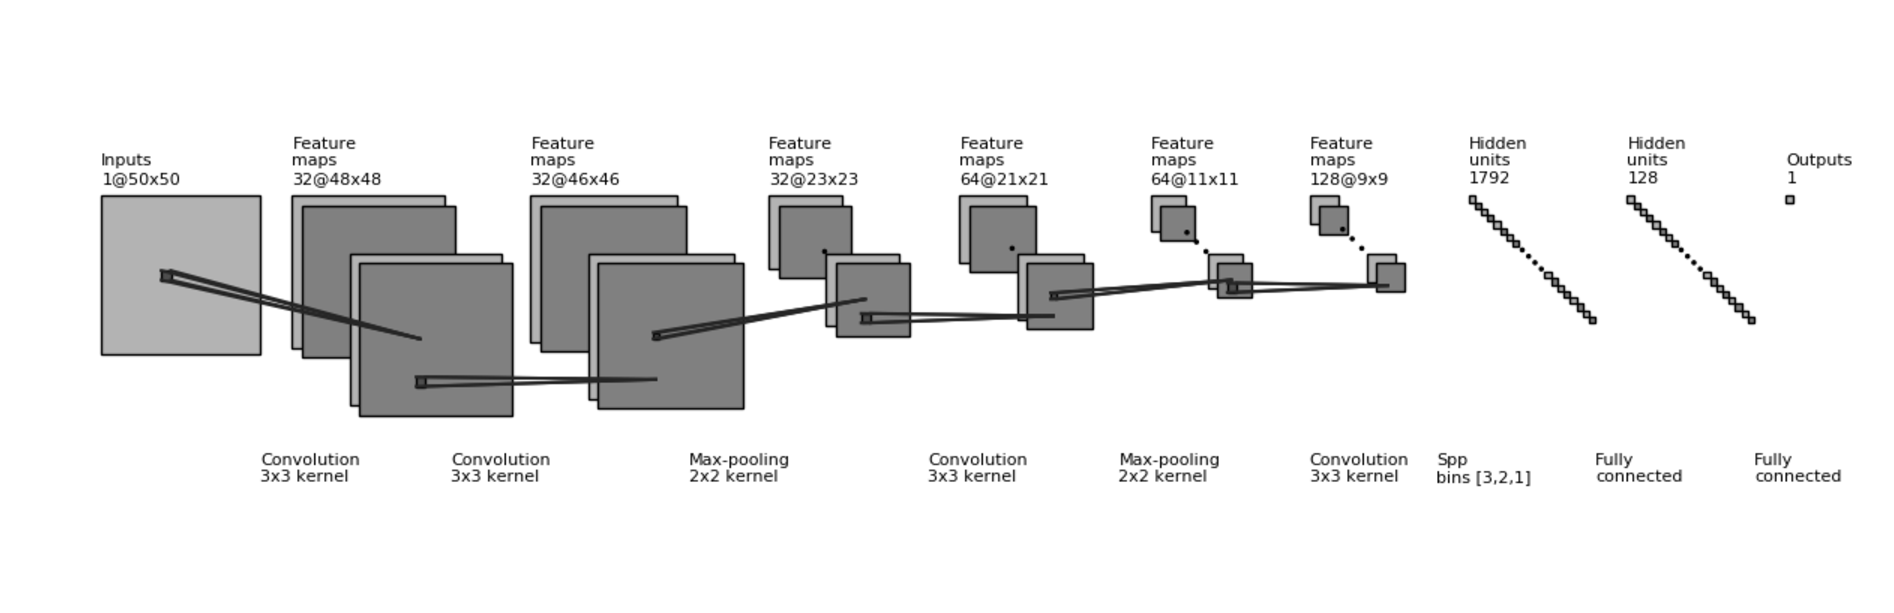
\includegraphics[scale=0.5]{mynet.eps}}
    \caption{我的网络结构示意}
    \label{fig:label}
\end{figure}
spp层是使用了动态尺寸的池化核将任意尺寸的输入池化到固定尺寸的输出。首先需要一个$BINS$来决定输出的尺寸,通常会选择多个输出尺寸来获得更多的信息。如输入图片尺寸为$x \times x$,需要的输出尺寸为$n \times n$,则计算
$$ksize = \lceil \frac x n \rceil$$
$$stride = \lfloor \frac x n \rfloor$$
再利用$ksize$和$stride$做最大池化。对$BINS$中每个输出尺寸都做了最大池化后,把这些数据排成一行输出到全连接层。\cite{spp}最开始是为了实现输入不同尺寸的图片到网络中进行训练所以想使用spp,但由于tensorflow的局限,一是如果输入不同尺寸的图片,就没法使用batch,只能每次输入一个图片;二是spp需要使用图片的动态尺寸,生成动态池化核来进行池化,但tensor自带的池化函数只支持静态池化核,需要自己重写池化函数,又遇到了使用tensor写循环语句的困难。考虑到图片伸缩对本问题的影响不大,故最后改为将输入单词图片都resize到$50 \times 50$,但仍然保留spp层。尽管spp层也需要每次输入的图片尺寸相同,但如果输入图片都变为另外一个尺度,网络也不需要改动,可以直接利用原网络。这样就可以实现多尺度维度的输入来提高效果。

相对于之前的LeNet,网络深度更深,输入图片尺寸的设计也更为灵活,连续使用了两个$3 \times 3$的卷积核来代替原来的一个$5 \times 5$的卷积核则是基于VGGNet的思想。

在损失函数上,考虑到我们的问题中精确度比较重要,故在损失函数中降低了正样本的比重。原本的损失函数为
\[\mathsf{targets} \times -\log(\mathsf{sigmoid}(\mathsf{logits})) + (1 - \mathsf{targets}) \times -\log(1 - \mathsf{sigmoid}(\mathsf{logits}))\]
新的损失函数为
\[\mathsf{targets} \times -\log(\mathsf{sigmoid}(\mathsf{logits})) \times \mathsf{pos\_weight} +(1 - \mathsf{targets}) \times -\log(1 - \mathsf{sigmoid}(\mathsf{logits}))\]
其中$\mathsf{targets}$为数据的标签,正样本为1,负样本为1,我们的数据中公式图片为正样本。$\mathsf{logits}$为网络的输出,经$\mathsf{sigmoid}$后为网络预测的为正样本的概率。$\mathsf{pos\_weight}$则是我们加入的一个比重,用来调节损失函数。当我们令这个比重小于1时,若网络的输入为正样本,则损失函数更小。

\section{CTPN的启发}
\noindent

在独立做完以上工作后,查阅论文时发现在OCR领域的一些文字识别的工作。如CTPN\cite{ctpn}、CRNN等。CRNN主要做的是文字识别工作,而CTPN做的是文字检测。

CTPN做的是自然场景图象中的水平文字检测,主要是在Faster RCNN的基础上结合双向LSTM生成的模型。首先是通过VGG提取特征,将生成的feature map经过一些处理后输入双向LSTM中,生成既包含CNN学习到的空间特征,也包含LSTM学习到的序列特征的特征图。再将特征图通过类似Faster RCNN的RPN网络,获得建议文本位置(text proposals)。CTPN生成的是宽度不变的anchor,通过寻找anchor中心和高度来获得一个小尺寸的建议文本位置,如图3.2,上面是传统的RPN的输出,下面为CTPN输出的建议文本位置,可以看见一个文本有许多小宽度的建议位置,接下来只需要通过文本线构造办法,将这些连接起来形成一个文本检测框。

\begin{figure}[hp]
    \centering
    
\includegraphics[scale=0.5]{rpn.eps}
    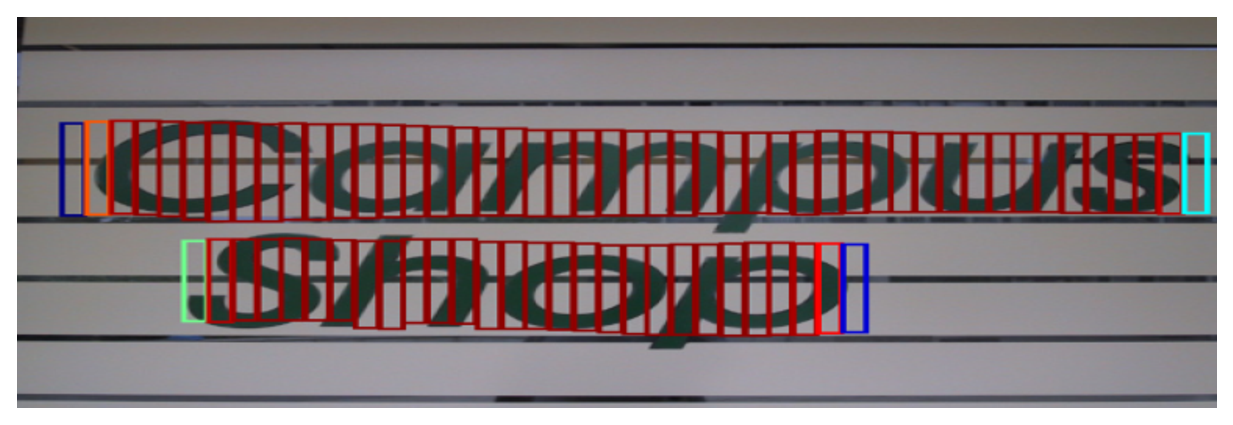
\includegraphics[scale=0.5]{ctpn.eps}
    \caption{CTPN proposals}
    \label{fig:label}
\end{figure}

CTPN的工作是自然场景图象中的文字检测,用在我们的论文图片中有大材小用的样子。但是CTPN的方法给予了我一些启发。在处理单词图片时我们直接将单词图片resize到了固定长宽。单词图片长宽比例很不均匀,若直接resize到方形,原本长宽比例很大的单词和长宽比例接近1的单词就显得不对等,而公式图片的特征变化更为明显。在CTPN中并不直接检测整个文本,而是一段一段地检测文本。故在处理图像时把长宽比大于2的单词分割为两个图片,前者长宽比为1比1,后者为剩下的,递归此操作,最终得到的图片长宽比都不大于2,这样再resize损失的特征大大减少。


